\documentclass[10pt, conference, compsocconf]{IEEEtran}

\usepackage[utf8x]{inputenc}
\usepackage[pdftex]{graphicx}
\usepackage{amsmath}  % for \hookrightarrow
\usepackage{xcolor}   % for \textcolor
\usepackage{listings}
\lstset{basicstyle=\ttfamily,
  showstringspaces=false,
  columns=fullflexible,
  frame=single,
  commentstyle=\color{red},
  keywordstyle=\color{blue},
  breaklines=true,
  postbreak=\mbox{\textcolor{red}{$\hookrightarrow$}\space},
}

% correct bad hyphenation here
\hyphenation{op-tical net-works semi-conduc-tor}

\newcommand{\niklas}[1]{{\textbf{[Niklas says: #1]}}}

\begin{document}

\title{Implications of Conducting Internet of Things Experimentation in Urban Environments}

\author{
\IEEEauthorblockN{Lasse Steenbock Vestergaard}
\IEEEauthorblockA{Smart Urban Designer\\
The Alexandra Institute\\
Aarhus, Denmark\\
lasse.vestergaard@alexandra.dk}
\and
\IEEEauthorblockN{Niklas Kasenburg}
\IEEEauthorblockA{Machine Learning Specialist\\
The Alexandra Institute\\
Copenhagen, Denmark\\
niklas.kasenburg@alexandra.dk}
\and
\IEEEauthorblockN{Morten Skov Jørgensen}
\IEEEauthorblockA{Senior Cyber-Physical Specialist\\
The Alexandra Institute\\
Copenhagen, Denmark\\
morten.skov@alexandra.dk}
}

\maketitle

\begin{abstract}
Cities are constantly evolving, and are turning into hackable environments optimized for IoT experimentation. In this article, we tap into this movement in order to investigate practical implications of utilizing these kinds of environments when performing IoT experiments. We have conducted \textit{in the wild} research through deploying a Wi-Fi tracking infrastructure at two Danish festivals, and have performed quantitative analysis on the collected data. From running the experiments, in a non-laboratory setting, we found that hackable urban environments are interesting platforms for testing IoT technologies. Our findings also suggest that mundane aspects like access to power grids as well as availability and appearance of the build environment can have significant impact on the results of urban IoT experimentation. More generally, this suggest that cities are not hackable by default, and they need to be thoroughly designed and optimized for IoT in order to ensure successful experimentation.

\end{abstract}

\begin{IEEEkeywords}
IoT; Wi-Fi; Tracking; Cultural Events; Prototyping; Hacking; Experimentation; Smart City

\end{IEEEkeywords}

\IEEEpeerreviewmaketitle

\section{Introduction}

Tinkering with Information Technology (IT) and developing prototypes is happening everywhere, and is becoming a basic skill, as well as an approach when diving into uncharted technical territories. In parallel to this, cities are subject to similar movements, and are now being portrayed as ever changing domains that are never complete - they are perpetual betas. Consequently, cities are turning into dynamic environments that are fostering and even encouraging hacking and prototyping~\cite{Fredericks2019}.

City authorities have started to exploit the possibilities unfolding from cities being temporary, adjustable and hackable and they are promoting cities as test beds and environments for experimentation~\cite{Latre2016}. Cities are constantly being augmented with new IT infrastructures (e.g. Wi-Fi, Low Power Wide Area Networks (LPWAN) and intelligent lamp posts), advancing possibilities for experimentation -- we now talk about cities as platforms for hacking. In addition, infrastructures are being prepared for deploying all kinds of temporal equipment like sensors, screens, interactive installations etc. By adopting the notion of city as a platform, the urban environment becomes a common ground between hackers and authorities, where they can synergize on city development through a combination of top-down and bottom-up approaches~\cite{Mulder2019}. In our research, we are following the trend of hackable cities~\cite{2019}, and are investigating how to utilize such platforms for conducting urban experiments. We are approaching this arena from a technically oriented Internet of Things (IoT) \cite{Ghasempour2016} prototyping perspective, and are especially interested in the practical implications that emerge when hacking the urban environment.

Even though we are tapping into the hackable city movement, we have chosen not to focus on actual cities as our physical testing ground. Instead we have perceived festivals as temporal cities. A festival has the same basic infrastructure elements like electricity grid, water supply, draining systems and waste management. It often has residential areas (camping areas), shopping areas and leisure zones (including concert areas). Last but not least, festivals represent physical areas with a high concentration of moving and interacting people~\cite{Jarvis:2013:USW:2494091.2499216}. City centres usually experience a constant flow of people traversing the streets, but the concentration of people is governed by factors such as day of week, time of day, city events and season. Consequently, it can be challenging to find the optimal occasion for conducting IoT experiments like tracking people. Furthermore, obtaining permission to conduct an IoT experiment in a city centre, can be time consuming due to bureaucratic city administrations. While it depends on the actual aim of a specific experiment, we wanted to test Wi-Fi tracking abilities in crowded environments. Additionally, we needed a critical amount of tracking data in order to make reliable post-analysis. Adding up these prerequisites, the focus was moved towards festivals instead of conventional cities, as we concluded that the likelihood of experiencing an optimal environment was higher in a physically confined environment.

From an overarching perspective, this article is investigating the potential of IoT prototyping in urban environments. We want to find out if state-of-the-art IoT technologies (specifically Wi-Fi dongles and Raspberry Pis) can be reliably utilized under prototyping conditions in urban settings in order to understand practical implications of temporarily deploying IoT prototypes in such settings.

In the remainder of the article we initially introduce related work. Then we elaborate the research methodology, and describe the technical setup, of the prototyping environment, including data analysis considerations. This is followed up by a case study from two festivals in Denmark, and finally we discuss practical learnings.

\section{Related Work}

Through our investigations, we have come across research on urban experimentation, where especially~\cite{2019} is central. The authors emphasize city hacking as a platform for tinkering and experimenting for the greater good of cities and citizens at large. The pivot point is mainly addressing hackability as a tool for engagement and collaboration, and not the actual technical implications of conducting experiments. Others address learnings from conducting actual urban experiments and practical implications~\cite{Amaxilatis2018}. Their focus is primarily related to a specific experimentation platform developed during a three year EU project, and does not address the implications of utilizing the built environment. Other research is focusing on aspects like Maker cultures, where emphasis is put on the design approach surrounding the developed artefacts rather than the practical testing and resulting implications~\cite{9780071821131}. Nevertheless, practical technical implications have been addressed and e.g.~\cite{Longo:2017:CDC:3155100.3093895} have elaborated the need for calibrating sensors and managing the issues of poor measurement quality.

From the technical perspective, we have encountered examples of tracking people's movement. These utilize a number of different technologies to uniquely identify a person. Some novel approaches use behavioral features, such as gait~\cite{gait} or face recognition~\cite{face}. Others rely on cybernetic interfaces such as mobile phones or beacons to track people. Included in this term we see examples of using GPS chips in the phone~\cite{gps}, Bluetooth signal~\cite{bluetooth} or Wi-Fi probe requests~\cite{wifihubei,wifiuti,wifimonitor}.
In our research, we have utilized the latter to extrapolate information from the collected data. Finally, we are leveraging the methodology from~\cite{semantic} to make segmentations based on features extracted from spatial and temporal information about devices~\cite{largescalemonitoring, monitorflows}.

\section{Methodology}

Our research has been conducted following a \textit{research in the wild} approach, meaning that we have gone out of the laboratory, and performed our investigations directly in a real setting \cite{Chamberlain2012}. More specifically, we attended two festivals in Denmark during the summer of 2018, where we were deployed our Wi-Fi sensors. During the festival (including construction/deconstruction) we have generated quantitative as well as qualitative data. We have generated quantitative data through collecting anonymized tracking data from the Wi-Fi sensors. Qualitative data has been generated through our own notes, and experiences from setting up, running, and taking down the prototyping equipment.

\subsection{Technology Use} \label{technology use}
Technically, we have used off-the shelf hardware combined with state-of-the-art software components to develop sensors and collect data. Throughout the article we use the terms \textit{device} and \textit{sensor} for describing two different elements in our setup. Device refers to external sources such as mobile phones and laptops (the entities we are tracking). Sensor refers to our hardware (trackers) we deployed during the festivals (the entities that collect data from devices).

To physically collect MAC addresses of devices, we utilized Raspberry Pi’s with an external omnidirectional Wi-Fi antenna and 4G dongles for connectivity. The external Wi-Fi antenna was a D-Link 150 High-Gain USB Adapter, which has been tested to be able to gather MAC addresses in a radius of 40 meters in perfect conditions e.g. open fields and no interference. We used a mix of Raspberry Pi 2 and Raspberry Pi 3 models, both running Raspbian, and on both models we used the same software packages. For transmitting the data, a Huawei E3372h 4G dongle was used to provide connectivity to our server where analysis was conducted. The software running on the Raspberry Pi’s was a combination of Node.js and bash commands. We utilized the TCPDump \cite{tcpdump} command available in Raspbian OS with certain flags to put the Wi-Fi interface in monitor mode and only look at the probe requests.

To comply with the current legalistic standards in Denmark \cite{blip}, the MAC addresses were put through a SHA256 hash function, which renews the salt every 24 hours at 2 a.m., to ensure that the data cannot be used to track people over multiple days. The second responsibility of the software was to normalize the data before sending it to the server. This included a dBm value, a timestamp, the hashed MAC address as well as a flag indicating if a given mobile devices is spoofing it’s MAC address, using the 7’th bit in the OUI octet of the MAC address. The latter gives us the possibility to distinguish between spoofed and non-spoofed devices, or universally administered addresses (UAA) and locally administered addresses (LAA)~\cite{spoofing}.

\subsection{Data processing} \label{sec:dataproc}
The collected data went through pre-processing to reduce noise, filter out irrelevant data, anonymize data and perform feature extraction prior to the data analysis. The first pre-processing steps include restricting the data to the festival interval (from 3 a.m. of the first day to 2 a.m. of the day after the festival), removing data created by the Wi-Fi antennas of our sensors and round the timestamps to 30 seconds. Since there can be multiple datapoints for the same device at the same timepoint, we use the one with the dBm closest to zero, i.e. closest to the device whose signal was recorded.

We can use this data to count how many devices have been seen at a defined time-interval (not smaller than 30 seconds) and location and visualize it in form of a timeline. However, when looking at movement of visitors, we need to remove spoofed data, data from stationary devices and other spurious data. Therefore, and since we were interested in information about every device, i.e. visitor, we extracted features for every unique hash, i.e. device, similarly to~\cite{largescalemonitoring}: 1) The time a device was at the festival. This is computed by the difference of the timestamp of first and last record of this device ignoring intervals without a record, larger than or equal to 2 hours. 2) Number of unique sensors a device has been seen at 3) Number of times a device has switched between sensors 4) Whether the device was seen in a restricted area, where only employees and volunteers have access.

\subsection{Data filtering} \label{sec:filtering}

\begin{figure}[tb]
  \centering
  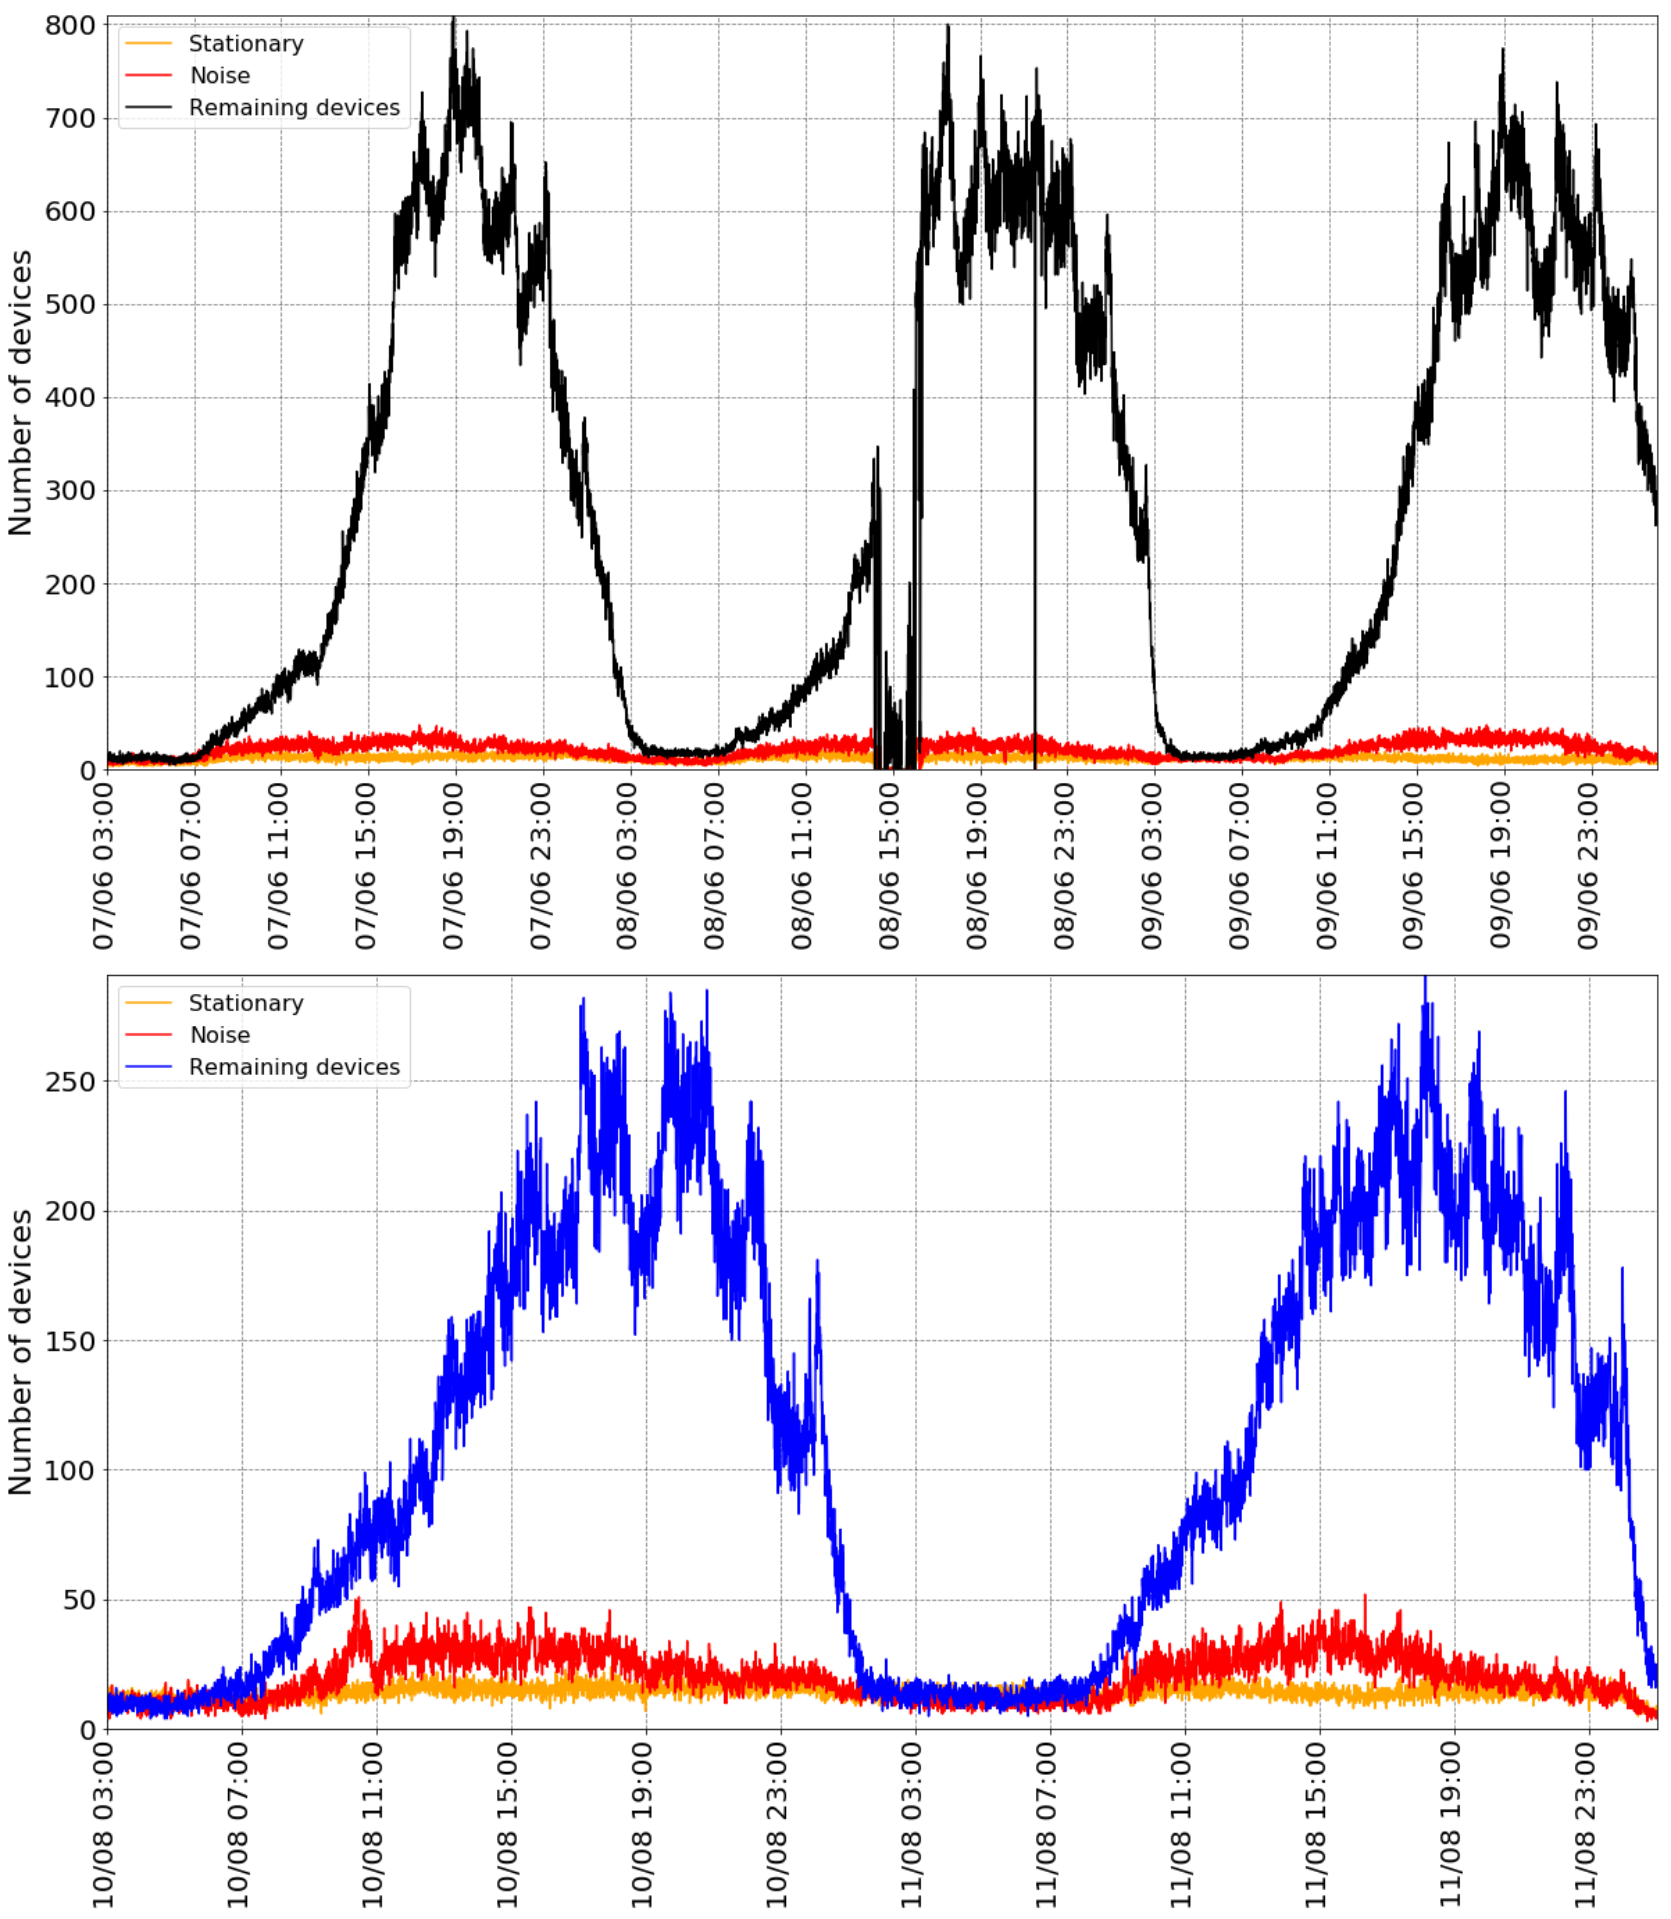
\includegraphics[width=\linewidth]{figs/stationary_noise.png}
  \caption{Number of stationary devices (orange), devices considered noise (red) and remaining devices (Northside: black, Haven: blue) as timeline over the festival days in 30 second steps. Stationary devices were tagged based on number of sensors they have been seen at ($<3$) and number of hours they where at the festival ($>14$). Noise devices were tagged based on number of sensors they have been seen at ($<3$) or number of minutes they where at the festival ($<5$).}
  \label{fig:stationary_noise}
\end{figure}

It is necessary to remove data that was recorded from signals sent by stationary devices, so that only signals from mobile devices are kept. Stationary devices that can be present at the festival are laptops used by the employees or volunteers, Wi-Fi access points or mobile phones of employees and volunteers located at the same place (typically entrance or food/drink booth) for several hours.  

Unlike~\cite{largescalemonitoring} we do not have access to the MAC address, but only to a hash. We can therefore not use it to filter devices based on the hardware producer. Instead we used an approach similar to~\cite{monitorflows}. We assume that devices seen at few sensors ($<n_{stat}$) and for a long period of time ($>t_{stat}$) are stationary. Note that using $n=1$ can be too small if the granularity is fine enough for a stationary device constantly being recorded by multiple sensors.

In addition to stationary devices, many devices are only seen at few sensors ($<10\%$ of the total amount of sensors) or only for a short period of time (only a couple of minutes). It is questionable that this data can be used to learn something about the movement of visitors. We therefore decided to remove devices which have been seen at less than $n_{noise}$ sensors or for less than $t_{noise}$ minutes.

We chose the following settings: $n_{stat}=n_{noise}=3$, $t_{stat}=14$ hours, and $t_{noise}=5$ minutes.
These were selected after a visual inspection of timeline graphs showing the number of devices over time (see Figure~\ref{fig:stationary_noise}) for a set of chosen values for $n_{stat}$, $n_{noise}$, $t_{stat}$ and $t_{noise}$, so that the amount of stationary and noise devices is approximately constant~\cite{largescalemonitoring} and a reasonable amount is filtered out. Values for this grid search were based on ad-hoc experience.

\section{Case study} \label{cases}
During the summer of 2018 we were given access to two major music festivals in Denmark, namely Northside Festival \cite{northside} and Haven Festival \cite{haven}, located in Aarhus and Copenhagen respectively. Both festivals address younger adults between 20 and 40 years of age.

Northside Festival is the third-largest festival in Denmark with 40.000 guests during a three-day event, which have been held for the last ten years. It is held every year in Aarhus, and attracts large crowds with an average age of 33 years and 55\% women vs 45\% men~\cite{avgagens}. It strives "[...] to create the most innovative and sustainable music event" \cite{nscore} and is a major player on the European festival scene. The festival is designed with two large central stages overlooking the main area, a smaller third stage in a smaller area, and a small tent stage for intimate events. It also has minor "chill out" areas scattered around the main area for off loading, when people want to step away from the music. 

Haven Festival is a, comparatively, smaller festival in Copenhagen with 7.000 guests during a two-day event, which has been held since 2017. It has been created by members from The National, Mikkeller and Claus Meyer who "have teamed up to create new experiences from their own art forms, namely beer, food, art, and music, bringing these ingredients together at one festival"~\cite{havenabout}. The festival is designed with two main stages overlooking the main area with a view over the harbor of Copenhagen. It also consists of two smaller areas with minor stages and areas to escape the main music.

When conducting our experiments, sensors were placed in bars, food stands and other areas of interest, depending on the possibilities at the given festival. The locations were decided by points of interest in conjunction with the hypothesis’ given by the festival management and the realistic possibilities during the festival, such as location of current infrastructure, e.g. power outlets and buildings to place the sensor in and on. From earlier experiments \cite{aiexperiments}, it was noted that the average time between a device sends a probe request is 35 seconds and as such, a person would be able to ”skip” one sensor if moving at a normal walking speed \cite{walkingspeed} of 1.4 m/s between multiple sensors. 

\subsection{Case analysis}
After removing spoofed data and other devices with a single record, we detected 16571 unique devices during the festival period of Haven and 28328 devices during the festival period of Northside. Of these 109 (0.7\%) were deemed stationary and 8804 (53.1\%) noise in the Haven data, while 167 (0.6\%) were deemed stationary and 8041 (28.4\%) noise in the Northside data (see Section~\ref{sec:filtering} and Figure~\ref{fig:stationary_noise}). The data of the remaining 7738 devices recorded for the Haven festival and 20239 devices recorded at Northside was used in the analysis.  

For a basic analysis we looked at the number of unique devices, i.e. visitors, over time at a chosen stage together with the occurrence of a concert at the same stage. Figure~\ref{fig:stage_timelines} shows that the number of visitors indeed correlates with the concert time, peaking during the concert and decreasing afterwards. In addition, we see an expected increase of visitors before the start of each festival day towards the first concert and an expected decrease after the last concert of each day.

\begin{figure}[tb]
  \centering
  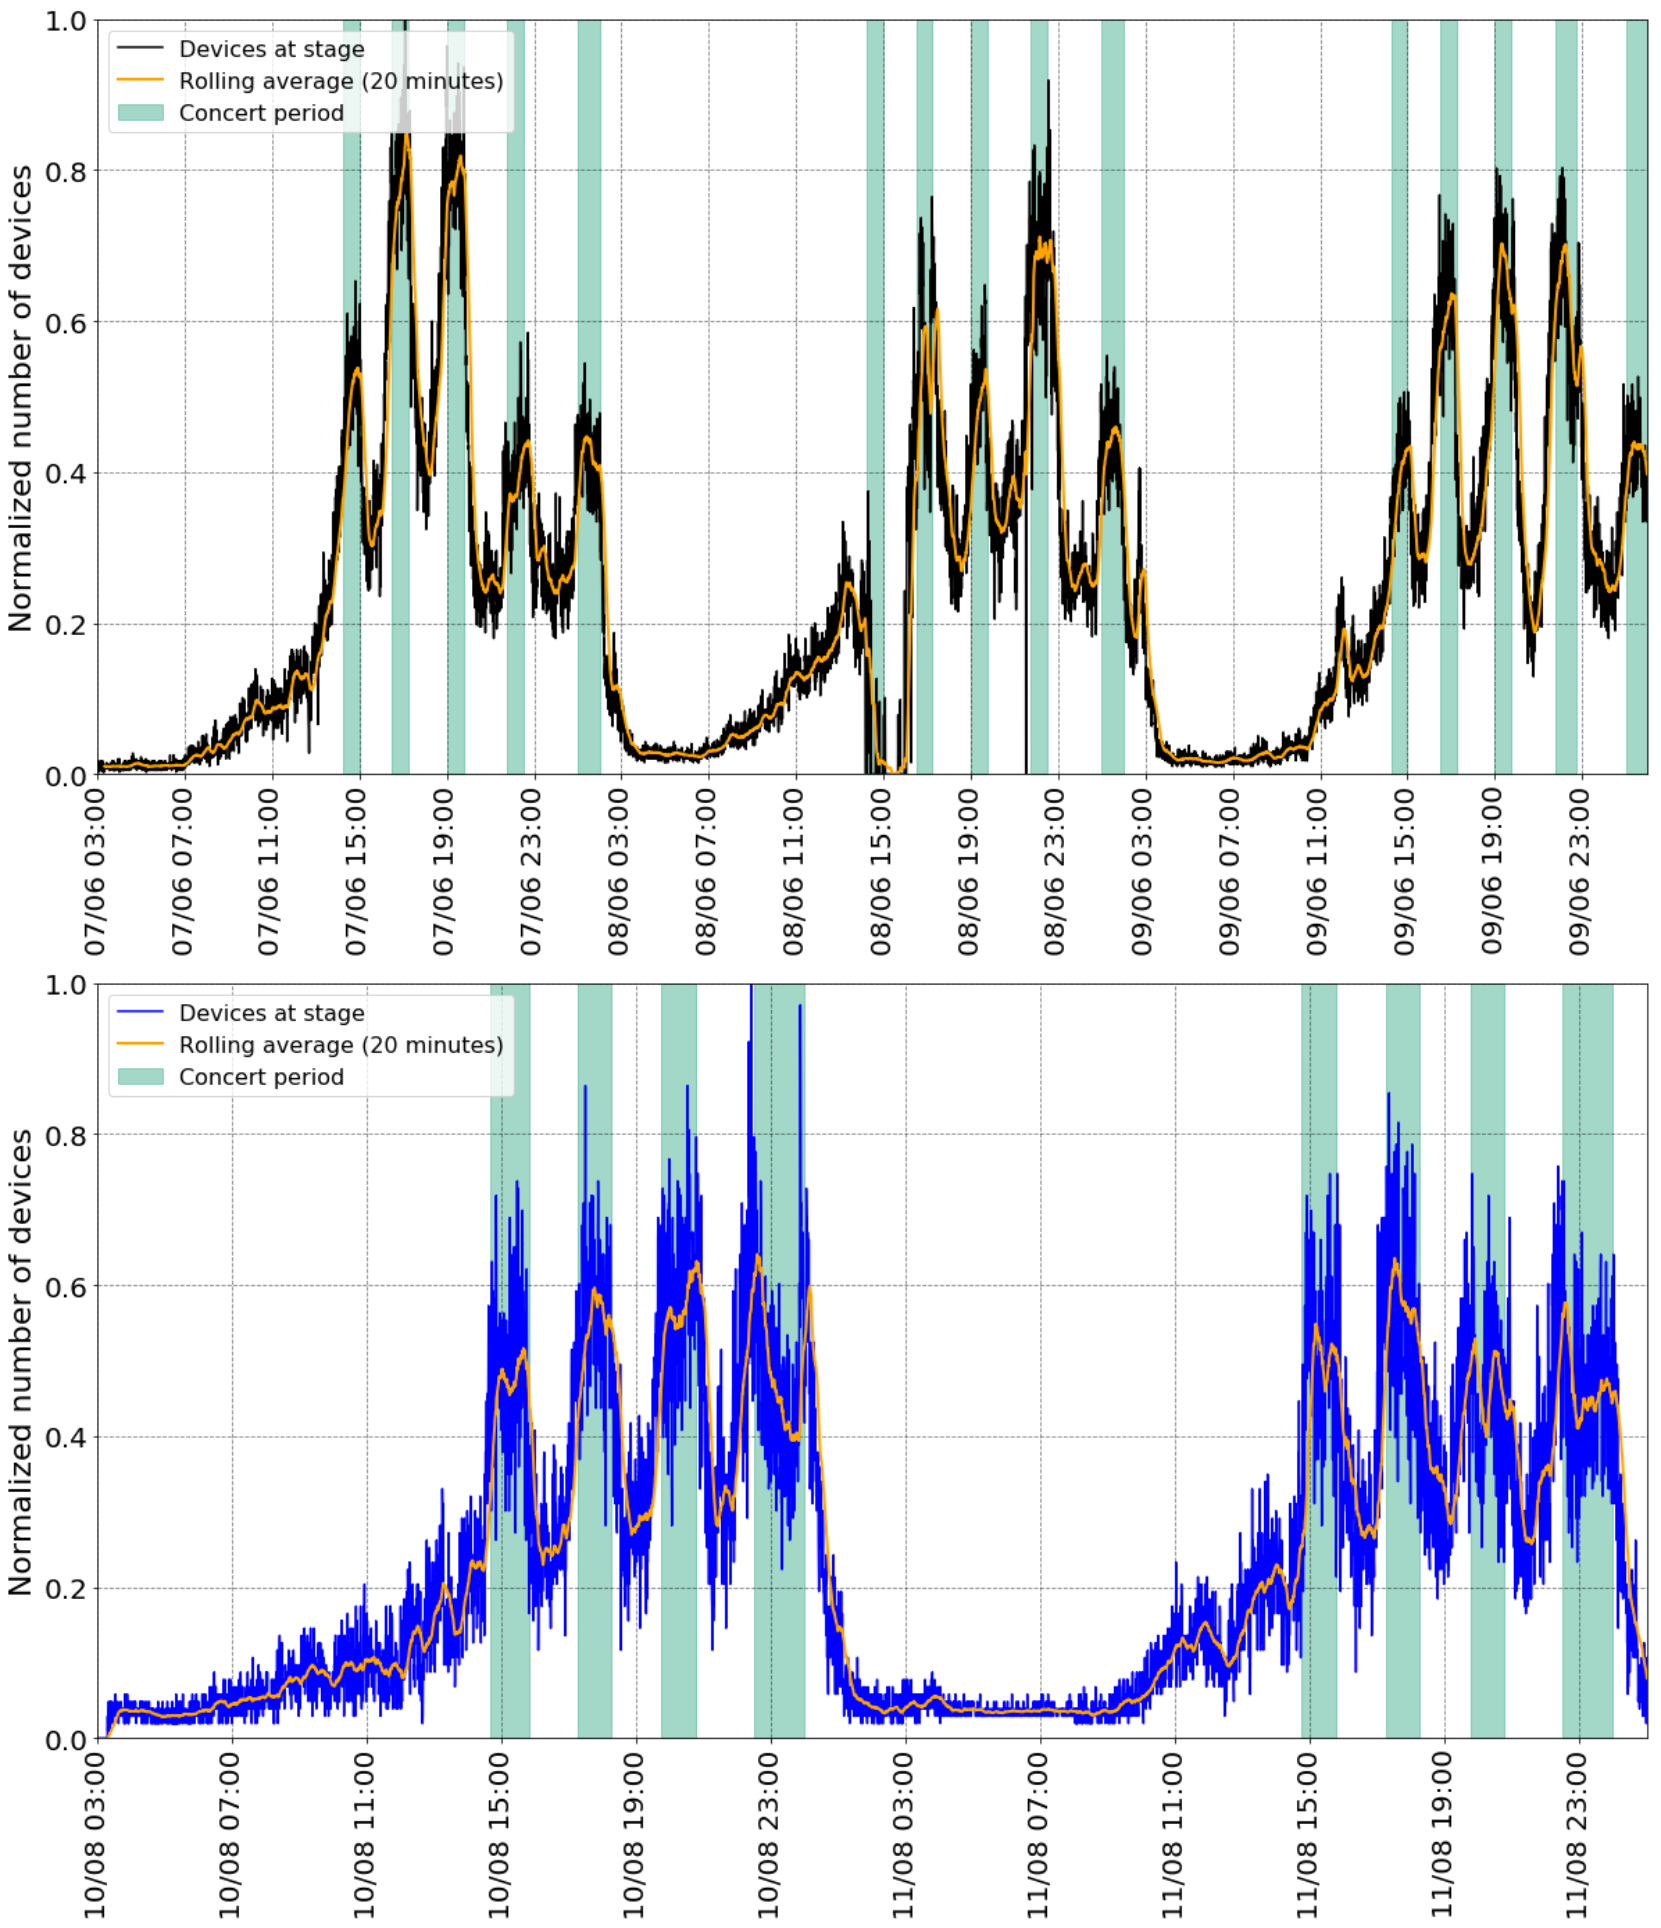
\includegraphics[width=\linewidth]{figs/stage_timelines.png}
  \caption{Amount of devices (Nortside: black, Haven: blue) at a chosen stage throughout the festival period in 30 seconds steps normalized to be between 0 and 1. The orange line shows the average of devices over the past 20 minutes. The shaded areas denote the periods during which there was a concert at the corresponding stage.}
  \label{fig:stage_timelines}
\end{figure}

Figure~\ref{fig:features} A--C show the distribution of three computed features (see Section~\ref{sec:dataproc}) in form of a boxplot over all visitors for both festivals separately. While 75\% of the visitors at Northside stayed at least 3.6 hours, at Haven only 60\% stayed that long. Similarly, only 25\% of Haven's visitors stayed more than 7.2 hours, while almost half (46\%) of Northside's visitors stayed longer than that. This can be explained by the different size of the festivals, Haven's close location to Copenhagen's city center and exceptionally bad weather during Haven causing visitors to leave the festival.

Beside differences in visiting time, it is also possible to see differences of the sensor set-up. Visitors at Northside where seen at more sensors (13 on average) and switched more often between them (40 times on average) than at Haven (seen at 8 sensors and switched 29 times on average). This means we had a better coverage and granularity at Northside festival than at Haven.

\begin{figure}[tb]
  \centering
  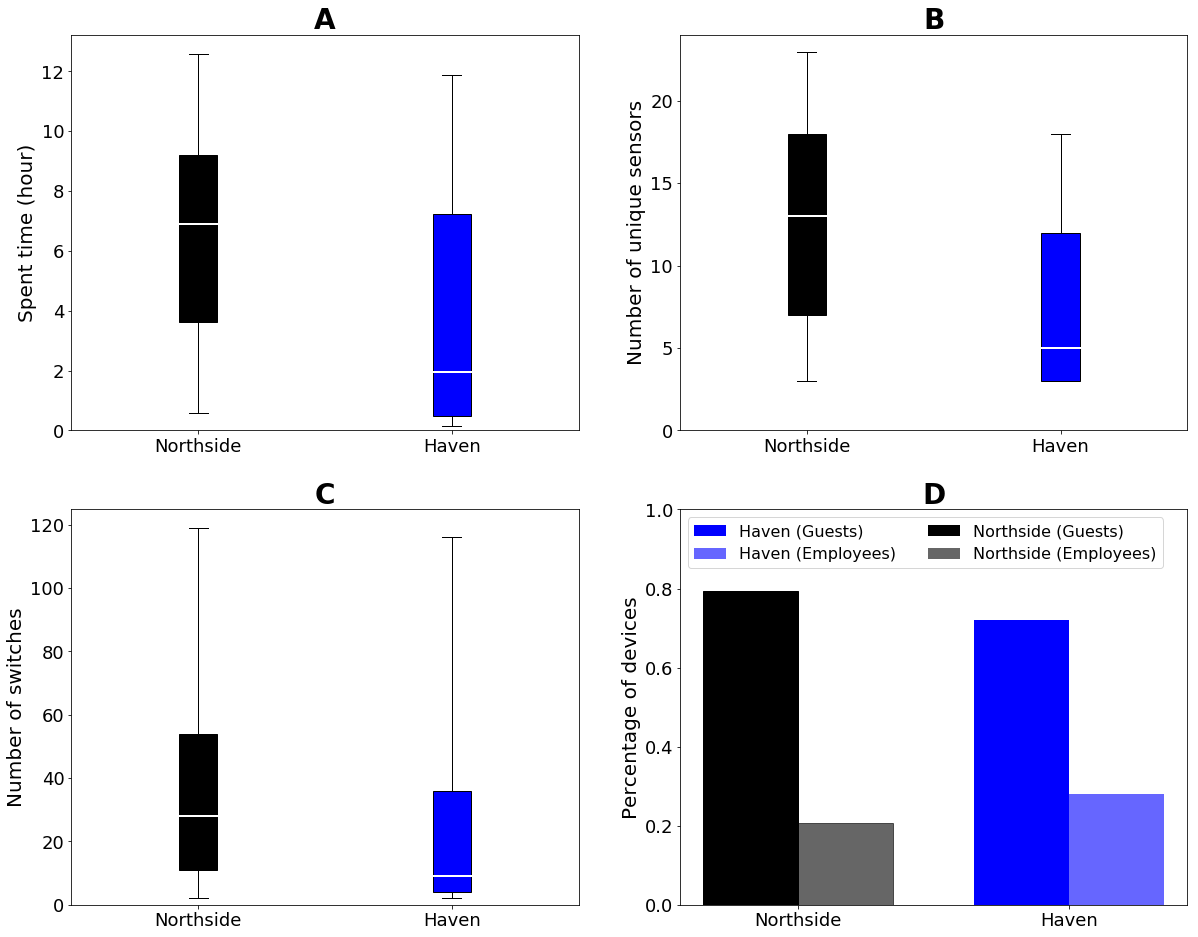
\includegraphics[width=\linewidth]{figs/features_boxplot.png}
  \caption{\textbf{A--C}: Boxplots showing the distribution for the three device features (\textbf{A} spent time, \textbf{B} number of sensors, \textbf{C} number of switches) over all visitors at Northside (black) and Haven (blue). Marked are the 5\% (lower whisker), 50\% (white line) and 95\% (upper whisker) percentile. \textbf{D}: Amount of guests (solid bar) and employees or volunteers (transparent bar) in percentage for both Northside (black) and Haven (blue).}
  \label{fig:features}
\end{figure}

\section{discussion}
Through our tracking experiments we encountered several challenges which affected the quality of the technical setup as well as the following data analysis. From the physical setup perspective, we had to make compromises which were assisted by the fact that the festival granted a unique access to festival grounds and installations including power grid.

For both festivals two challenges were encountered that made it imperative to make some informed choices: Firstly, it was decided to use 4G dongles to avoid any issues with the festival’s own wired infrastructure. This decision was twofold: 1) If the festival experienced any issues with their connectivity it could inflict badly on the data gathering. 2) The sensors could run the risk of introducing potential problems in the Point-Of-Service setup that could have devastating effects on the festival's economy. Secondly, the physical layout of the festivals gave rise to some challenges as both festivals have large vacant areas in the center of the grounds to afford audiences a better view of stages and move about, which hamstrung the effort to position the sensors in the optimal locations. This resulted in a loss of granularity and coverage, but could not be avoided unless dedicating significant resources to setting up e.g. battery stations. We therefore focused on the accompanying elements, such as bars, food stands, access areas and toilets as our major focal point.

During Northside Festival, we decided against collecting spoofed data points as it was assumed that this could jeopardize the system’s ability to handle the flow, which was expected to include around 40.000 devices inside the range of normal opening hours. Our hypothesis was validated, when activating spoofed data for a short time span during peak hours at the festival, which resulted in a break down (see label '08/06 15:00' in Figure~\ref{fig:stationary_noise}). Collecting and transmitting all this data could pose a threat to stability of the servers as well as create buffering issues on the devices as the 4G dongles had a limit, especially with many people in the vicinity, using their mobile phones. During Haven Festival, a much lower number was expected and was deemed possible for the system to handle this pressure, and therefore the collection of spoofed Wi-Fi data points was activated to facilitate further post-analysis on these. 

From the data analysis perspective we learned that finding a good trade-off between coverage and granularity, and having both at a high enough level is essential to be able to analyze how visitors move around at the festival area. Nevertheless, it is possible to remove uninformative or spurious data when using sub-optimal setups. Furthermore, being able to group the devices into guests and employees (see Figure~\ref{fig:features} D) can be helpful to perform a different analysis per group. This, however, would require that sensors are set up in areas where only employees or volunteers have access to distinguish those devices from the rest.

The overarching learnings suggest that the physical layout of the festivals seems to be the culprit for our poor results. This further indicates that relatively mundane aspects like access to physical infrastructures can have significant impact on the ability to conduct IoT experiments in urban environments. Going back to the idea of hackable cities, this is an interesting movement with the ability to revolutionize real- and large-scale IoT prototyping through an \textit{always on} platform accessible for anyone independently of affiliation and available economic resources. In order to unlock the real potential, we argue that cities are not hackable by default, but they need to be carefully designed and reshaped in order to enable high quality experimentation which again feeds into collaborative city-making.

\section{Conclusion}
In this article we have been focusing on practical learnings from conducting IoT prototyping in hackable urban environments. We have specifically emphasized festival settings, the technical setup, data analysis and general learnings. The state-of-the-art IoT technology we have utilized in our research has performed as expected, and did not, in itself, result in major breakdowns during the deployment phase. We did learn that the physical infrastructure of the festivals were challenging because Wi-Fi tracking was not taken into account when designing the festival layout. Additionally, the settings were optimized for best audience experiences, and not hacking in general. These aspects are evident in our post data analysis, and made it challenging to conduct high quality analysis due to holes in data as well as difficulties tracking devices across the entire festival area. We experienced noisy data due to sub-optimal locations of Wi-Fi trackers (e.g. near exits and thereby collecting data from bypassers outside of the festival premise). 
Even though the quality of the hardware and software were sufficient, it is important to note that the overall quality of our data could have been better. This was mainly due to a discrepancy between the hypotheses from the festivals and the feasibility of the physical environment to cover these. This goes to show that we need to design future hackable cities carefully, and on a practical level, be able to support placement of equipment in a multitude of ways as to support different types of experiments as the physical location can have great impact on the results.

% use section* for acknowledgement
\section*{Acknowledgment}
The research has been supported by the Innovation Fund Denmark and we want to thank Northside and Haven festivals for letting us hack their physical infrastructures and especially their IT team for assisting us in doing so.

\bibliographystyle{IEEEtran}
\bibliography{IEEEabrv,ref}

\end{document}


